% Application paper (provisional venue IEEE CCWC 2027). Limit: 7 pages with references.
% Abstract numbers repeat Section VI (t3-h evaluation, docs/experiments.md).
% Uses the standard IEEE conference class without margin or font overrides.
\documentclass[conference]{IEEEtran}
\usepackage{cite}
\usepackage{amsmath,amssymb}
\usepackage{booktabs}
\usepackage{graphicx}
\usepackage{url}
\usepackage[hidelinks]{hyperref}
\hypersetup{pdftitle={Application Paper Draft: Task-Space Imitation Learning for Lunchbox Packing},pdfauthor={}}

\title{A Task-Space Imitation Learning System for Robotic Lunchbox Packing}
\author{\IEEEauthorblockN{Author 1}}

\begin{document}
\maketitle

\begin{abstract}
Hotel, event, and airline catering repeatedly place specified food items into
compartmented containers on fixed schedules. We present an imitation learning
system that teaches this lunchbox-packing task to a six-joint RB5
collaborative robot from demonstrations given with a seven-joint RB-Y1 leader
arm. Because the two arms cannot be matched joint to joint, the leader's wrist
motion is mapped, relative to a clutch press, to the follower's tool position
in cylindrical coordinates about the base axis, and one command-shaping stage
limits the commands in both teleoperation and autonomous execution. The
platform adds a parallel gripper and three RGB cameras; demonstrations are
converted into a LeRobot dataset, and an Action Chunking with Transformers
(ACT) policy predicts Cartesian position targets and gripper commands.
Trained on 140 demonstrations, the policy packs a model carrot and two snack
packages into a black box and the two holes of a meal box in a fixed order.
In 30 trials over six source layouts, it completed 22 packings and placed 73
of 90 items correctly, with no item released into a wrong compartment and a
median completion time of 66.6~s. The remaining failures arose in grasping,
mainly retries that drifted away from the item.
\end{abstract}

\begin{IEEEkeywords}
robotic manipulation, teleoperation, task-space imitation learning,
lunchbox packing, system integration
\end{IEEEkeywords}

\section{Introduction}
\label{sec:intro}
% Fig. 1 placed here so that it appears at the top of page 2 (two-column floats go to the next page).
\begin{figure*}[t]
\centering
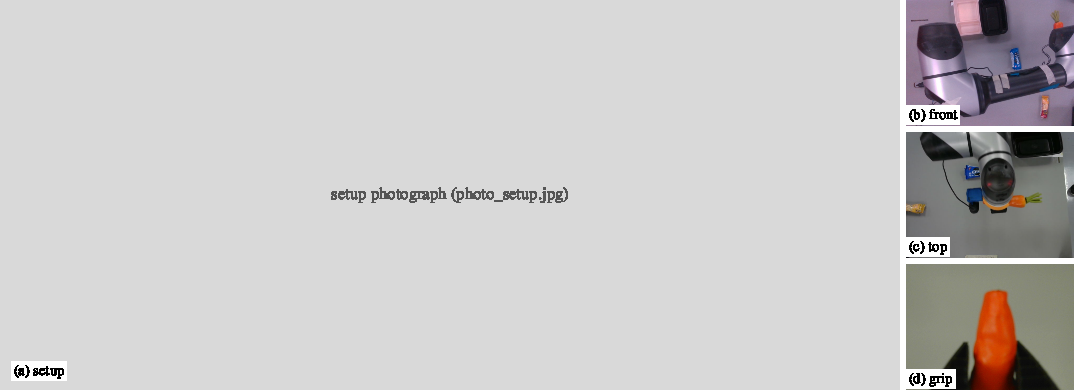
\includegraphics[width=\textwidth]{figures/fig1_setup.pdf}
\caption{(a) Experimental setup. (b)--(d) The front, top, and grip camera views
at one moment of a demonstration, just after the carrot was grasped. The front
and top cameras are fixed; the grip camera moves with the gripper.}
\label{fig:setup}
\end{figure*}
% Made by paper/figures/make_fig1.py: camera frames from data/demos/real_20261029_123638/episode_001 (640 x 480,
% 1.5 s after the first close); setup photo paper/figures/photo_setup.jpg (placeholder until it exists).
Hotels, event venues, and airport catering services must prepare many meals
consistently and in time for scheduled service~\cite{venetian2026menu,gategourmetcatering},
which involves repeatedly placing specified food items into the compartments
of containers. A useful packing system must complete the whole sequence of
picking, transferring, and placing several items, not a single grasp: an item
dropped during transfer or released into the wrong compartment leaves the
lunchbox incomplete. This motivates an approach in which operators teach the
packing motions through demonstrations and the resulting behavior is assessed
at the level of the complete task.

Visual imitation learning provides a way to learn such motions from images
and demonstrated actions. Action Chunking with Transformers
(ACT)~\cite{zhao2023act} shows how predicting sequences of actions supports
manipulation from visual input.
Applying a learned policy requires a demonstration-to-execution workflow in
which camera observations, measured robot states, and commanded actions have
consistent representations and explicit timing. We study this integration on
a three-item task: a model carrot goes into a black box, and two packaged
snacks, an Oreo and a RITZ, go into the large and small holes of a meal box,
in a fixed order. The policy must therefore tell the snacks apart by sight to
choose the compartment.

Our hardware introduces a further integration requirement: the RB-Y1 leader
arm has seven joints, whereas the RB5 follower has six. Their different
kinematic structures do not admit direct one-to-one joint copying. We use
leader forward kinematics and a clutch-relative mapping in cylindrical
coordinates about the follower's base axis to command the follower's tool
position. This separates the operator's arm configuration
from the Cartesian target delivered to the RB5 and allows demonstrations
to be collected with the available leader hardware. The resulting policy
still uses follower-specific state observations; the task-space interface
serves demonstration collection and execution on the RB5.

This paper presents an imitation learning system for robotic lunchbox
packing. An ACT policy predicts absolute Cartesian position targets and
gripper commands from images and follower state, and the gripper orientation
follows a predefined rule. The contributions are:
\begin{enumerate}
\item An integrated platform connecting a kinematically dissimilar leader
and follower, multi-view visual observations, and gripper control for a
lunchbox-packing application.
\item A demonstration-to-deployment workflow that preserves the Cartesian
position and gripper action representation across episode recording,
dataset conversion, ACT training, and autonomous command execution.
\item A real-robot evaluation of 30 trials over six source layouts, scored
per item in four stages, which shows reliable placement and locates the
remaining failures in grasping and in retries absent from the demonstrations.
\end{enumerate}
In these trials, the policy completed 22 of 30 packings and placed 73 of 90
items correctly, with no item released into a wrong compartment. The study is
scoped to these three items, fixed containers, source layouts within the
demonstrated region, and a predefined packing order.

\section{Related Work}
\label{sec:related}
\subsection{Robotic Food Serving and Packing}
Tanemoto et al.~\cite{tanemoto2022bento} developed a household bento-serving
system that combines food and environment recognition, dialogue, information
storage, goal generation, and manipulation using tools. Their work places
food serving within a complete household-assistance task. Santos et
al.~\cite{santos2024packing} collected virtual-reality demonstrations of
packing irregular grocery-like objects and learned a Markov model for
predicting packing order. We focus instead on executing demonstrated
pick-and-place motions on a physical manipulator under a prescribed order and
compartment assignment.

\subsection{Interfaces for Demonstration Collection}
ALOHA~\cite{zhao2023act} uses approximately scaled leader and follower arms
with joint-space mapping to collect bimanual manipulation demonstrations.
Universal Manipulation Interface (UMI)~\cite{chi2024umi} uses handheld grippers
for demonstration collection and combines a relative-trajectory action
representation with inference-time latency matching to support deployment
across robot platforms. In our setup, the seven-joint leader and six-joint follower are connected
through a task-space teleoperation interface that maps the leader's wrist
motion to the follower's tool position in cylindrical coordinates about the
base axis. Demonstrations are recorded
while the RB5 executes the task, and the policy uses its joint and gripper
state together with RGB observations. Policy transfer across follower robots
is outside the scope of this study.

\subsection{Visual Imitation Learning for Manipulation}
ACT~\cite{zhao2023act} learns action chunks from visual observations and robot
state using a transformer-based conditional variational autoencoder, with
temporal ensembling of overlapping predictions. Diffusion
Policy~\cite{chi2023diffusion} models action sequences through conditional
denoising and executes them with receding-horizon control. Mandlekar et
al.~\cite{mandlekar2022offline} show that learning from human demonstrations
depends on demonstration quality, algorithmic choices, and the criteria used
to select policies for evaluation; we therefore document the dataset and
evaluation conditions. We use ACT unchanged; our focus is the connection
between data collection, action representation, robot execution, and
task-level evaluation.

% Section III: System design and implementation (target 1.30 pages with Table I, Fig. 1, Fig. 2).
% Sources: docs/hardware.md, configs/real.yaml (real-1 final, frozen), docs/decisions.md
% (real-1, grip-5, rec-1, rec-6, hw-1). Data format and ACT execution details: Section IV.
\section{System Design and Implementation}
\label{sec:system}

\subsection{Hardware and Workspace}
\label{sec:hardware}
The follower is a six-joint Rainbow Robotics RB5-850 collaborative
manipulator. A host computer sends commands to its control box and receives
the robot state over two TCP channels through the vendor's Python API.
The operator uses the right arm of an RB-Y1 leader with seven Dynamixel joints.
Its handle carries a clutch button, a mode button, and an analog trigger.
The leader is read without torque while the clutch is pressed. When the
clutch is released, its joints are torqued to hold their pose. The end
effector is an in-house 3D-printed parallel gripper driven by one Dynamixel
MX-106 actuator on a separate serial bus.

Three RGB cameras record at $640\times480$ and 30~fps: a RealSense D435
fixed obliquely in front of the workspace (\emph{front}), a Logitech C270
fixed above the item area and looking straight down (\emph{top}), and a
Logitech Brio~101 mounted on the gripper and aimed at the fingers
(\emph{grip}). Exposure, gain, and white balance are fixed. Each exposure is a
multiple of 1/120~s, so the 60~Hz room lighting does not flicker in the images.
At start-up, each camera's mean brightness is compared with a reference value,
and a deviation above 15\% requires operator confirmation.
Depth is not used. A black box and a meal box with a large and a small hole
are fixed at marked positions on the robot's table, and the items are placed
within the view of the top camera (Fig.~\ref{fig:setup}). Table~\ref{tab:hardware}
summarizes the components and operating settings.
% TODO: item dimensions, finger clearance, hole sizes, container positions in the base frame.

\begin{figure}[t]
\centering
\fbox{\parbox[c][0.55\columnwidth][c]{0.95\columnwidth}{\centering
Photograph placeholder: RB5-850 with gripper and grip camera, RB-Y1 leader,
front and top cameras, black box, meal box (large and small holes), item area.}}
\caption{Experimental setup. The front and top cameras are fixed; the grip
camera moves with the gripper.}
\label{fig:setup}
\end{figure}

\begin{table}[t]
\caption{Hardware, Software, and Operating Settings}
\label{tab:hardware}
\centering
\footnotesize
\setlength{\tabcolsep}{3pt}
\begin{tabular}{@{}lp{0.68\columnwidth}@{}}
\toprule
Item & Specification\\
\midrule
Follower & RB5-850, 6 joints; control box software 8.4.4\\
Leader & RB-Y1 right arm, 7 joints (XM540/XM430), 2~Mbps\\
Gripper & In-house parallel, MX-106, current-based position mode\\
Cameras & D435 (front), C270 (top), Brio~101 (grip); RGB $640\times480$, 30~fps\\
Host & Intel i7-13700H, NVIDIA RTX A1000 6~GB laptop GPU, Ubuntu 24.04\\
Software & rbpodo 0.16.14, LeRobot 0.6.1, PyTorch 2.11\\
Command loop & 50~Hz Cartesian targets (\texttt{move\_servo\_l})\\
Speed limits & 250~mm/s in $r$ and $z$, 360~mm/s along $\phi$;
J1 75~deg/s, J2--J6 60~deg/s; 2.5~m/s$^2$\\
Workspace & $r$ 250--800~mm (depends on $z$), $z$ 19--465~mm,
$\phi$ $-160$ to $133^\circ$\\
Gripper force & 0.50~A current cap while moving, 0.84~A while grasping\\
\bottomrule
\end{tabular}
% TODO: TCP offset, tool mass, and collision-detection setting used in the evaluation
% (the TCP offset on the controller is still provisional; docs/hardware.md).
\end{table}

\subsection{Software Architecture}
\label{sec:architecture}
All software runs on the host as Python processes, arranged in a recording
path and an autonomous-execution path that share the camera, gripper, and
command-shaping components (Fig.~\ref{fig:architecture}).

In the recording path, a teleoperation process runs a 50~Hz cycle.
In each cycle, it reads the leader joints and the latest RB5 state,
computes the follower target, and sends it.
The gripper runs in its own 50~Hz thread, so a gripper fault does not stop
the arm. The cameras run in a separate process with a capture thread and a
writer thread per camera, which store every frame as a JPEG image with its
capture time. Image work therefore cannot delay the command cycle. Robot,
gripper, and camera samples are stamped with the same monotonic clock and
saved at their native rates. The 30~Hz dataset is built from them offline
(Section~\ref{sec:workflow}).

In the execution path, a policy process opens the same cameras with the same
fixed settings and runs ACT on the GPU, at most once per 30~Hz step. Each
predicted action chunk is stamped with its observation time. A servo
process keeps the 50~Hz cycle without waiting for the policy. It combines the
chunks by time and passes the resulting target through the same command
shaping as in teleoperation. The two processes are pinned to separate CPU
cores. The stated rates are implementation targets, not hard real-time
guarantees. A cycle whose command would be sent more than 30~ms after the
previous one keeps the previous target, and three such cycles in a row stop
the run.

\begin{figure}[t]
\centering
\fbox{\parbox[c][0.62\columnwidth][c]{0.95\columnwidth}{\centering
Diagram placeholder.\\[3pt]
Recording: leader FK $\rightarrow$ clutch-relative cylindrical mapping $\rightarrow$
command shaping $\rightarrow$ \texttt{move\_servo\_l} (50~Hz); gripper thread;
camera process (30~fps JPEG); logs with one clock $\rightarrow$ 30~Hz dataset.\\[3pt]
Execution: cameras + robot state $\rightarrow$ ACT (policy process, GPU)
$\rightarrow$ time-stamped chunks $\rightarrow$ servo process (50~Hz) $\rightarrow$
same command shaping $\rightarrow$ \texttt{move\_servo\_l}; gripper thread.}}
\caption{Recording and autonomous-execution paths. Both send absolute
Cartesian targets through the same command shaping; the recorded action is
the shaped target.}
\label{fig:architecture}
\end{figure}

\subsection{Dissimilar Leader--Follower Interface}
\label{sec:interface}
The leader's joint angles are converted into the position of its wrist
center $\mathbf{p}_L=(x_L,y_L,z_L)$ by forward kinematics on the vendor's URDF
model, with $x_L$ pointing forward and $z_L$ up.
The seven leader joints and the six follower joints are never matched one to
one. The follower target is expressed in cylindrical coordinates
$(\phi, r, z)$ about the RB5 base axis: azimuth, horizontal distance from the
axis, and height. When the clutch is pressed at time $t_0$, the interface
stores $\mathbf{p}_L(t_0)$ and the current target $(\phi_0, r_0, z_0)$. Each
axis of the leader displacement $\Delta\mathbf{p}_L=\mathbf{p}_L(t)-\mathbf{p}_L(t_0)$
then drives a single follower coordinate. In the normal mode,
\begin{equation}
\phi = \phi_0,\quad r = r_0 + s\,\Delta x_L,\quad z = z_0 + s\,\Delta z_L,
\label{eq:normal}
\end{equation}
and while the mode button is held,
\begin{equation}
\phi = \phi_0 + k\,\Delta y_L,\quad r = r_0,\quad z = z_0,
\label{eq:rotate}
\end{equation}
with $s=1$ and $k=0.3^\circ$/mm. The commanded position is
$\mathbf{p}_d=(r\cos\phi,\ r\sin\phi,\ z)$ in the base frame. Releasing the
clutch freezes the target, and the next press re-anchors both references, so
the operator can reposition the hand without moving the robot.

Early teleoperation trials used a Cartesian mapping,
$\mathbf{p}_d=\mathbf{p}_d(t_0)+s\,\Delta\mathbf{p}_L$. In these trials, the
natural arcs of the operator's hand leaked into unintended follower axes, and
sideways drift turned the base. With \eqref{eq:normal} and
\eqref{eq:rotate}, forward and backward leader motion moves the gripper along
the arm's radial direction, vertical motion changes only its height, and the
base turns only in the rotate mode. A dead band
of 0.3~mm and a first-order low-pass filter with a 30~ms time constant
suppress encoder-step jitter of $\mathbf{p}_L$.

The tool orientation is not teleoperated. Roll and pitch keep the ready-pose
values, with the gripper pointing straight down. The yaw changes with the
target azimuth $\phi$, so the gripper turns with the arm and the follower's
last joint stays still. The orientation is thus a fixed function of the target
position, and the position together with a gripper value fully specifies the
command. Items must therefore be graspable without wrist rotation.

The gripper opening is proportional to the trigger. At start-up the gripper
follows only after the trigger reaches its current opening, which prevents
a jump. In current-based position mode, the motor current is limited to
0.50~A while moving. When the fingers stall on an item, the goal is set
60~ticks ($5^\circ$) past the stall point and the cap is raised to 0.84~A,
so the item is held firmly.

\subsection{Operating Limits and Robot Interface}
\label{sec:limits}
In every 20~ms cycle, the desired position passes through a fixed sequence of
command-shaping stages. Equations \eqref{eq:normal} and \eqref{eq:rotate}
give this position in teleoperation; a policy action gives it in autonomous
execution. The first two stages use the same cylindrical coordinates as
the mapping.
\begin{enumerate}
\item \emph{Workspace}: the target is clipped to
$r_{\min}(z)\le r\le r_{\max}(z)$, $19\le z\le465$~mm, and
$-160^\circ\le\phi\le133^\circ$ (Table~\ref{tab:hardware}). The lower
height bound keeps the fingers just above the table.
\item \emph{Speed}: the component of each step along $\phi$ is limited to
360~mm/s, and the component in $r$ and $z$ to 250~mm/s. The target may lag the
hand by up to 20~mm and catches up after the hand stops.
\item \emph{Singularities and joint limits}: the joint angles of the step are
predicted by the RB5's analytic inverse kinematics. Wrist, shoulder, and
elbow singularities and joint limits are monitored. Near one of them, the
speed limit falls linearly to 25\%; closer still, the step is not sent.
\item \emph{Joint speed}: per-joint limits of 75~deg/s for J1 and 60~deg/s
for J2--J6.
\item \emph{Acceleration}: a 2.5~m/s$^2$ limit on the target, applied
last. In trials, the largest accelerations occurred when an earlier limit
switched on or off.
\end{enumerate}
The shaped position and the orientation rule form the TCP pose that is
streamed to the controller with the RB5 API call \texttt{move\_servo\_l}.
In one teleoperation trial, the arm followed the commands about 80~ms
behind, and the joint error stayed within $0.23^\circ$. The speed limits
were raised step by step from 100~mm/s, based on hand speeds measured in
logged real-robot trials. They were then frozen together with all other
teleoperation settings before demonstration collection.

Before any motion, the software checks that the controller is in real mode
and that its TCP offset matches the expected value. It moves the robot to a
fixed ready pose at low joint speed only after the operator types a
confirmation. During operation, stale robot state, repeated leader read
failures, or repeated late cycles stop the robot.
The limiter is not collision avoidance and offers no formal safety
guarantee. No collision-aware planner is used, and the controller's
internal motion generation is outside the scope of this paper.
% TODO: state the controller collision-detection setting and tool mass used in the evaluation.


% Section IV: Demonstration collection and policy deployment (target 1.10 pages with Table II).
% Sources: docs/data_rules.md, docs/experiments.md, docs/decisions.md (rec-1, rec-6, p3-a, p3-b, t3-a .. t3-e),
% session folders data/demos/real_* (episodes.json, notes.txt), configs/policy.yaml, checkpoint config.json.
% Evaluation placements, trials and success criteria: Section V.
\section{Demonstration Collection and Policy Deployment}
\label{sec:workflow}

\subsection{Task and Demonstration Protocol}
\label{sec:protocol}
One episode packs all three items in a fixed order: the carrot into the black
box, then the Oreo into the large hole and the RITZ into the small hole of the
meal box. A fixed order gives one correct action at every moment, whereas a
free order would let the policy average between choices. Before each episode,
the items are placed at random positions within the view of the top camera,
not touching each other or the containers. Which item lies nearest the robot
also varies, so the order must be inferred from the item types rather than from
their positions. Each item is oriented so that the fingers close across it
without wrist rotation. The operator starts each episode with the gripper
open, from a different pose within about 10~cm of the ready pose.

Every item is handled with the same sequence: approach above it, descend
vertically, close, lift, move above the target, lower slightly, open, and
lift. After the last item, the operator brings the gripper back above the
item area, near the ready pose, and ends the episode there; this pose is also
where the next episode starts. The operator moves steadily, without hesitation or searching. An episode is
discarded when an item drops or lands outside its target (including the wrong
hole), when anything is hit, when the motion pauses for more than about 2~s,
or when a camera reports an error. A natural re-grasp after a slip is kept
if the episode still ends correctly. Episodes end with a keyboard key or at a time
limit (180~s for three items), and every session is checked with the converter before the next one
begins.

\emph{Recovery demonstrations.}
A pilot policy that saw only successful grasps closed beside an item, lifted
the empty gripper, and carried it to the box. The gripper position cannot
reveal the miss, because the soft items and an empty grasp both leave the
fingers nearly closed, and the motor current rises in only some of the real
grasps (Section~\ref{sec:interface}); only the grip camera shows the miss
reliably. Recovery episodes
therefore contain one deliberate miss: the operator closes beside an item,
lifts the empty gripper, pauses for 0.5--1~s so that the grip camera sees the
empty fingers, opens, moves directly above the item, and continues as in a
normal episode. In the three-item recovery set, each item is missed eight times,
covering four directions on the table. The miss lies 2.5--15.6~cm from the
following grasp (median 8.5~cm, center to center), and the empty lift is
8--15~cm.

\emph{Collection stages.}
Data were collected in stages, so that each policy's failures could motivate
the next set (Table~\ref{tab:datasets}). The first stages placed the carrot
and one snack per episode, normal (2N) and with recovery (2R). A policy trained
on them had no demonstrated action once both snacks lay on the table, so all
later episodes contain all three items: normal (3N) and recovery (3R). The
earlier episodes remain valid under the same rule as scenes with one snack
absent. The evaluated policy is trained on the union of the four sets,
\emph{all} (140 episodes). Of 66 attempts in the three-item normal session, 51
were kept, and 7 of these include a natural re-grasp. Cameras, lighting,
container positions, and teleoperation settings were the same in every session.

\begin{table}[t]
\caption{Demonstration Sets and Training Datasets}
\label{tab:datasets}
\centering
\footnotesize
\setlength{\tabcolsep}{4pt}
\begin{tabular}{@{}llrrr@{}}
\toprule
Set & Content & Episodes & Frames & Mean (s)\\
\midrule
2N & Carrot + one snack, normal & 49 & 70{,}550 & 48.0\\
2R & Carrot + one snack, recovery & 16 & 24{,}862 & 51.8\\
3N & Three items, normal & 51 & 89{,}899 & 58.8\\
3R & Three items, recovery & 24 & 43{,}272 & 60.1\\
\midrule
all & 2N + 2R + 3N + 3R & 140 & 228{,}583 & --\\
\bottomrule
\end{tabular}
% Frames at 30 Hz; mean = frames / episodes / 30. Names in docs/experiments.md: 2N = u1, 2R = u2,
% 3N = u4n, 3R = u4r, all = u4 (u4a = u1 + u2 + u4n, an intermediate training set, not evaluated).
\end{table}

\subsection{Observation, Action, and Dataset Preparation}
\label{sec:dataset}
The state and the action at time step $t$ are
\begin{align}
 \mathbf{s}_t &= [q_{1,t},\ldots,q_{6,t},\,g^{\mathrm{pos}}_t],\\
 \mathbf{a}_t &= [x^{\mathrm{cmd}}_t,\,y^{\mathrm{cmd}}_t,\,z^{\mathrm{cmd}}_t,\,g^{\mathrm{cmd}}_t],
\end{align}
where $q_{1..6}$ are the measured follower joint angles in degrees, $g^{\mathrm{pos}}$
is the measured gripper opening, $(x,y,z)^{\mathrm{cmd}}$ is the shaped TCP
target in millimeters in the base frame (Section~\ref{sec:limits}), and
$g^{\mathrm{cmd}}$ is the trigger command. Both gripper values range from zero
(closed) to one (open). The label is thus the target that the robot was
commanded to reach, not its measured motion; the orientation follows from
the position by the rule of Section~\ref{sec:interface} and is not learned.
The observation adds the three camera images. Because the joint angles are
part of the observation, the policy is specific to the RB5.

A converter builds the dataset from the raw logs on a 30~Hz grid starting at
each episode's start. Targets and joint states, recorded at 50~Hz, are
interpolated to the grid times. For each camera, the frame captured nearest to
each grid time is used; in the four collection sessions, this frame lay within
17.6~ms of the grid time for 99\% of the samples. Episodes in which the clutch
was engaged for less than 1~s or the target moved less than 30~mm are left out,
as are episodes with camera gaps. The images are reduced from $640\times480$
to $320\times240$ with the same resampling function used at run time. The
result is stored in the LeRobot dataset format~\cite{cadene2024lerobot}, with
images as compressed video. Datasets from separate sessions are merged without
conversion, and each dataset keeps a copy of the settings used to build it.
% TODO: add the LeRobot entry (cadene2024lerobot) to references.bib.

\subsection{ACT Training and Autonomous Execution}
\label{sec:execution}
The policy is ACT as implemented in LeRobot~0.6.1. A ResNet-18 backbone
initialized from ImageNet encodes each camera image, and a transformer with
a 512-dimensional model and a conditional variational autoencoder (KL weight
10) predicts a chunk of 100 actions (3.3~s) from one observation. States,
actions, and images are normalized by their dataset mean and standard
deviation. Training uses a batch size of 8, a constant learning rate of
$10^{-5}$, and 100{,}000 steps, about 3.5 passes over \emph{all}. On the host's
laptop GPU this takes about 7~h. The checkpoint at the final step is
evaluated; no checkpoint is selected by test results.

At run time, the policy process predicts a new chunk from the latest images
and robot state whenever the previous inference has finished, at most once
per 30~Hz step. Each chunk carries the capture time of its observation. In
every 20~ms servo cycle, each recent chunk that covers the current time
contributes its action, interpolated between its 30~Hz steps, and the
contributions are averaged as in ACT~\cite{zhao2023act}:
\begin{equation}
\mathbf{a}(t) = \frac{\sum_{i} w_i\,\mathbf{a}^{(i)}(t)}{\sum_{i} w_i},\qquad
w_i = e^{-m i},
\label{eq:ensemble}
\end{equation}
where $i=0$ denotes the oldest chunk and $m=0.01$. Because the averaging is
done by time, a late or skipped inference only removes one chunk from the
average. The position passes through the command shaping of
Section~\ref{sec:limits}, and the gripper value goes to the gripper thread,
which applies the same grasp handling as in teleoperation.

The operator starts a run with a key after confirming the distance to the
first action. Inference runs only while the robot runs: each start clears the
old chunks and follows the first new one, because chunks predicted while the
arm stood still plan motion that did not happen. The robot holds its target when
the operator presses the hold key, when the newest chunk is older than 0.5~s,
when an action lies more than 100~mm from the current target, or when 180~s
have passed since the start; it stops when no chunk arrives for 3~s.


% Section V: Experimental setup and evaluation protocol (target 0.90 pages with the layout figure).
% Sources: docs/data_rules.md "Evaluation", docs/decisions.md t3-g (and addenda), configs/eval_layouts.yaml,
% data/eval/eval_sheet.csv. Results: Section VI.
\section{Experimental Setup and Evaluation Protocol}
\label{sec:experiments}

\subsection{Evaluated Policy and Source Layouts}
\label{sec:layouts}
The evaluation tests one policy: ACT trained on \emph{all} at its final checkpoint
(Section~\ref{sec:execution}), from a single training run. No comparison
condition is evaluated; the study measures whether the complete application
performs the packing task and how it fails.

The items are placed in five predefined source layouts
(Fig.~\ref{fig:layouts}). Each layout fixes the grasp point of every item in
the robot base frame, inside the region where items were grasped in the
three-item demonstrations (457--747~mm from the base axis), with the items at
least 21~cm apart and oriented as in the demonstrations. The layouts vary
which item lies nearest the robot: the carrot in two, the Oreo in one, and the
RITZ in two. In three layouts the RITZ lies nearer than the Oreo, so that
picking the nearest item first would break the packing order. The containers
stay where they were during data collection.

The table carries no marks. Instead, a top-camera photograph was saved for
each layout once its items were in place (Fig.~\ref{fig:layouts}). Before each trial, the execution
program shows the live top image with this photograph blended in and a circle
at each grasp point, located by an affine map from the base frame to the image
fitted to ten demonstrated grasps (rms error 18~px, about 2~cm on the table).
The operator places the items to match the photograph.

\begin{figure*}[t]
\centering
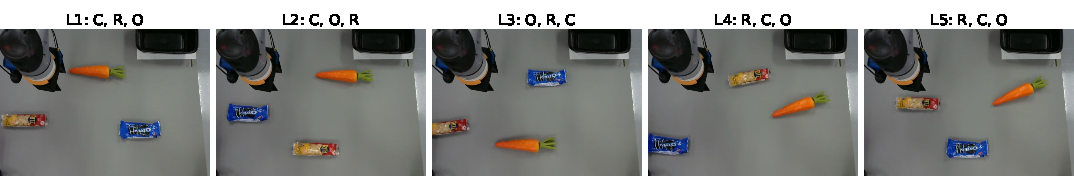
\includegraphics[width=\textwidth]{figures/fig_layouts.pdf}
\caption{The five source layouts, seen by the top camera in the photographs
used to place the items. Each label lists the items from nearest to farthest
from the robot base axis (C carrot, O Oreo, R RITZ). The gripper at the ready
pose is at the upper left and the black box at the upper right; the meal box
lies outside the view.}
\label{fig:layouts}
\end{figure*}
% Made by paper/figures/make_fig_layouts.py from data/eval/layouts/L*.jpg. Grasp points (x, y) in the base
% frame, mm (configs/eval_layouts.yaml): L1 C(80,-450) O(250,-690) R(-200,-600); L2 C(200,-480) O(-180,-580)
% R(100,-740); L3 C(30,-700) O(150,-460) R(-220,-640); L4 C(280,-620) O(-200,-680) R(60,-470);
% L5 C(250,-560) O(80,-720) R(-60,-560).

\subsection{Trial Procedure}
\label{sec:trials}
Each layout is tested four times, giving 20 trials in one session. Every round
visits all five layouts, and each round starts one layout later than the
previous one (L1--L5, then L2--L5 and L1, and so on), so that no layout is
always early or late in the session. Each trial is a separate run of the
execution program. The robot moves to the ready pose with the gripper open,
the operator places the items, and a single start key begins autonomous
execution. The operator then touches neither the items nor the robot. The trial
ends when all items have been released and the gripper has lifted, at the
180-s limit of Section~\ref{sec:execution}, or when the operator intervenes,
which counts as a failure. The controller settings are those of
Section~\ref{sec:limits}: collision detection at a 30\% threshold and a tool
mass of 0~kg.
Each trial leaves its own log of robot states, targets, gripper commands, and
inference times, together with a video of the three camera views whose frame
times are stored on the clock of the log.

\subsection{Success Criteria and Measures}
\label{sec:measures}
A trial is a \emph{complete success} when, within 180~s and without
intervention, the carrot rests in the black box, the Oreo in the large hole,
and the RITZ in the small hole, with the gripper open. The snacks are longer
than their holes, so a snack counts as placed when it rests touching the inside
of its hole, tilted or not; a snack on the rim does not. The criterion,
fixed before the trials, concerns the final state and does not require the
packing order, which is reported separately.

Each item is judged in four stages from the trial video: \emph{grasp} (lifted
off the table, including re-grasps within the limit), \emph{transport} (carried
above a container without dropping), \emph{place} (released and resting inside
some container), and \emph{correct} (that container is the assigned one). An
item that never reached a stage, such as the items left after the policy
stalled on an earlier one, is counted as not attempted there rather than as
failed. Each stage's rate is thus conditional on reaching the stage, which
locates the weak stage, while the share of the 60 items placed correctly shows
how early failures cascade. Borderline final states were decided by the
operator, who watched every trial.

The primary measures are the complete successes out of 20 with a Wilson 95\%
confidence interval~\cite{wilson1927probable}, the stage rates, the correctly
placed items out of 60, and the completion time of the successful trials, from
the start key to the last release. Failed trials are assigned a main cause and
excluded from the time statistics, so that fast failures do not appear
advantageous. Grasping is described by the share of items grasped at the first
close, the share of all gripper closes that lifted an item, and the recovery
rate: items grasped after at least one miss on them, over items with a miss.
An order error is recorded when an item is picked up and carried before an item
that precedes it in the packing order; releases into a wrong compartment are
counted separately. As a reference, the three-item demonstrations lasted
58.8~s on average (Table~\ref{tab:datasets}), measured from the start to the end
of recording rather than to the last release. Supporting measures are the
inference time, computed once per prediction, the servo interval, and the
number of late cycles and holds.
% TODO: add wilson1927probable (E. B. Wilson, J. Amer. Statist. Assoc., 1927) to references.bib.


% Section VI: Results and discussion (target 1.50 pages with Table IV and Fig. 3).
% Sources: data/eval/eval_sheet.csv (operator-confirmed judgments), data/policy/run_real_20261031_*.csv/.json/.mp4,
% docs/experiments.md (evaluation row), docs/decisions.md t3-g addendum 3.
\section{Results and Discussion}
\label{sec:results}

\subsection{Packing Performance}
\label{sec:performance}
Of the 20 trials, 12 were complete successes (60\%; Wilson 95\% interval
39--78\%), and 11 of these also kept the demonstrated order.
Table~\ref{tab:results} breaks the outcome down by item and by layout. Of the
60 items, 49 were placed correctly. No item was released into a wrong
compartment: every item that reached the place stage ended in its assigned
container, except one RITZ that came to rest on the rim of the small hole.
The losses occur earlier. The Oreo was lost mainly during transport (16 of 19
grasped Oreos reached a container) and the RITZ at the grasp (15 of 19
attempted). The carrot was grasped in 19 of 20 trials and then always placed;
the exception is the trial with an intervention.

The layouts differ more than the items. L1 and L4 succeeded in all four
trials with every item placed, whereas L2 and L3 succeeded once each. The
successful trials took a median of 54.1~s from the start key to the last
release (mean 56.9~s, range 40.4--82.6~s). The three-item demonstrations lasted
58.8~s on average under a longer measure (start to end of recording), so the
policy packs at roughly the pace of teleoperation rather than faster.
Fig.~\ref{fig:sequence} shows the fastest trial.

\begin{table}[t]
\caption{Evaluation Results (20 Trials)}
\label{tab:results}
\centering
\footnotesize
\setlength{\tabcolsep}{3.5pt}
\begin{tabular}{@{}lccccc@{}}
\toprule
\multicolumn{6}{@{}l}{(a) Stage rates per item, conditional on reaching the stage}\\
Item & Grasp & Transport & Place & Correct & Correct / 20\\
\midrule
Carrot & 19/20 & 19/19 & 19/19 & 19/19 & 19\\
Oreo & 19/20 & 16/19 & 16/16 & 16/16 & 16\\
RITZ & 15/19 & 15/15 & 14/15 & 14/14 & 14\\
\midrule
\multicolumn{6}{@{}l}{(b) Per layout}\\
Layout & Complete & \multicolumn{2}{c}{Correct items} & \multicolumn{2}{l}{Main failure causes}\\
\midrule
L1 & 4/4 & \multicolumn{2}{c}{12/12} & \multicolumn{2}{l}{--}\\
L2 & 1/4 & \multicolumn{2}{c}{9/12} & \multicolumn{2}{l}{RITZ not approached (2), rim (1)}\\
L3 & 1/4 & \multicolumn{2}{c}{6/12} & \multicolumn{2}{l}{Oreo displaced (3)}\\
L4 & 4/4 & \multicolumn{2}{c}{12/12} & \multicolumn{2}{l}{--}\\
L5 & 2/4 & \multicolumn{2}{c}{10/12} & \multicolumn{2}{l}{intervention (1), slip (1)}\\
\midrule
All & 12/20 & \multicolumn{2}{c}{49/60} & \multicolumn{2}{l}{}\\
\bottomrule
\end{tabular}
% One RITZ was not attempted (trial 20). Intervention: trial 5 (carrot re-placed by hand).
\end{table}

\begin{figure}[t]
\centering
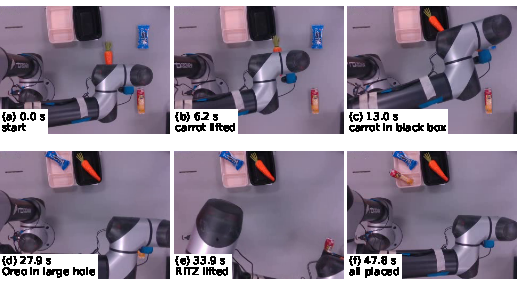
\includegraphics[width=\columnwidth]{figures/fig3_sequence.pdf}
\caption{A complete autonomous packing sequence (trial 18, layout L1), seen by
the front camera. Times are from the start key; the last release was at 40.4~s.}
\label{fig:sequence}
\end{figure}
% Made by paper/figures/make_fig3.py from data/policy/run_real_20261031_070212 (releases 9.4, 23.2, 40.4 s
% after the start key; resting items shown halfway between a release and the next close).

\subsection{Grasping and Recovery}
\label{sec:grasping}
Of the 59 attempted items, 29 were grasped at the first close. Grasping
again after a miss was common: after an empty close, the policy reopened,
moved above the item, and closed again, as shown in the recovery
demonstrations. In total, 24 of the 30 items with a miss were eventually
grasped (carrot 11/12, Oreo 7/8, RITZ 6/10). In the 12 successful trials, the
gripper closed 65 times for 36 items, 1.8 times per item. Over all trials,
only 54 of 181 closes lifted an item, but 94 of the closes came from the four
trials in which the policy stalled (Section~\ref{sec:failures}). No policy
trained without recovery demonstrations was tested under the same protocol, so
these numbers describe the evaluated policy and do not measure what the
recovery episodes contributed.

\subsection{Failure Analysis and Operational Behavior}
\label{sec:failures}
Eight trials failed. \emph{Items displaced from demonstrated states} caused
three, all in L3, where the Oreo lies nearest the robot. The fingers closed
on its edge; in two trials the Oreo was lifted and fell on the way, beside
the black box, and in the third it was pushed there without being grasped.
The policy then closed repeatedly at a fixed empty spot, every 5--6~s, until
the time limit, and neither the Oreo nor the RITZ was grasped. An item lying
next to a container never appears in the training data: episodes with a
dropped item were discarded (Section~\ref{sec:protocol}), and the recovery
episodes only show re-grasps near the item.
\emph{A far item not approached} caused two failures in L2. After placing
the carrot and the Oreo, the policy moved to an empty area about 25~cm from
the RITZ, which lay at the front edge of the item region, and stalled. The same
layout succeeded once, and in its fourth trial the RITZ ended on the rim of
the small hole. The remaining two failures occurred in L5. In one, the Oreo
was taken before the carrot, held near the fingertips, and slipped out on the
way. In the other, the gripper pushed the carrot and turned it to an
orientation that the fingers could not close across. The operator re-placed
it, so the trial counts as failed. Because the tool orientation follows a
fixed rule (Section~\ref{sec:interface}) rather than being learned, a rotated
item cannot be grasped.

The packing order was broken three times, all in L5: after missing or
displacing the carrot, the policy carried the Oreo first. The RITZ was never
carried before the Oreo. In L4, where the RITZ lies nearest, the first reach
went to the RITZ in all four trials; after missing it, the policy turned to
the carrot and completed all four trials in order. The order was therefore
learned, but proximity could take over when the next item in the order was
not grasped.

Execution was stable throughout. Over 54{,}167 predictions (28.2 per second),
inference took 23.6~ms at the median and 49.1~ms at the 95th percentile. The
servo interval had a median of 20.0~ms and a maximum of 40.3~ms, and 30 of
95{,}913 cycles were late. No hold was triggered, no robot state was stale,
and every run was closed with the operator's key, five of them after the time
limit; none ended with a controller stop.

\subsection{Application Scope and Limitations}
\label{sec:limitations}
The evidence comes from one policy, one training run, and one session; 20
trials leave a wide confidence interval. The layouts lie inside the
demonstrated item region, the items keep their demonstrated orientations, and
the containers, lighting, and model foods are fixed. Within this scope,
placement was reliable, and the limiting factors were grasping and continuing
from states the demonstrations do not cover. Demonstrations that pick up items
lying beside the containers, wider coverage near the robot and at the far edge
of the item region, and a perceived rather than fixed tool orientation are the
direct next steps. The task-space interface connects the dissimilar leader and
follower; it does not establish transfer to another follower. The study makes
no claim about real food, unseen objects, industrial readiness, or safety.


% Section VII: Conclusion (target 0.15 pages). Numbers repeat Section VI; no new claims.
\section{Conclusion}
\label{sec:conclusion}
This paper presented a task-space imitation learning system for lunchbox
packing in which a seven-joint leader arm teaches a six-joint collaborative
robot. A clutch-relative mapping in cylindrical coordinates and one
command-shaping stage serve
both teleoperation and autonomous execution, so the recorded action is the
target the robot executes. Trained with ACT on 140 demonstrations, one policy
completed 22 of 30 packing trials over six layouts and placed 73 of 90 items
correctly, with no item released into a wrong compartment and a median
completion time of 66.6~s. The failures arose in grasping, mainly retries
that drifted outward to the workspace bound and items flicked or pushed away
by the fingertips. Extending the data beyond the limits of
Section~\ref{sec:limitations}, and residual reinforcement learning, remain
future work.


\section*{Acknowledgment}
The images of the leader arm and of the RB5 in Fig.~\ref{fig:architecture} were
generated with ChatGPT (OpenAI, gpt-image) from photographs of our hardware.
% Required by IEEE: AI-generated content (text, figures, images, code) is disclosed in the acknowledgments.
% Provenance: C2PA records in paper/figures/photo_leader.png and photo_rb5.png.

\bibliographystyle{IEEEtran}
\bibliography{references}
\end{document}
